\documentclass{article}
\usepackage{natbib}
\usepackage{hyperref}
\usepackage{authblk}
\usepackage{fullpage}
\usepackage{color}

% \documentclass[fleqn,10pt]{wlscirep}
\usepackage[utf8]{inputenc}
\usepackage[T1]{fontenc}

% Additional Packages:
\usepackage{graphicx}
\usepackage[labelformat=simple]{subcaption}
\renewcommand\thesubfigure{(\alph{subfigure})}
\usepackage{amssymb}
\usepackage{amsfonts}
\usepackage{amsmath}
\usepackage{nicefrac}
\usepackage{textcomp} % For \textdegree (also try \usepackage{gensymb} which gives \degree)
\usepackage{soul} % For highlighting text

% Macro Definitions:
\def\s{\sigma}
\providecommand{\e}[1]{\ensuremath{\times 10^{#1}}}

% Keywords command
\providecommand{\keywords}[1]
{
  \vspace{5mm}
  \small
  \noindent
  \textbf{Keywords:} #1
  \normalsize
}

\title{Automated data-driven symbolic modeling of the lift forces acting on
flapping wings}
\date{}

\author[1]{Charles Richter} \author[2,3]{Hod Lipson} \affil[1]{Cornell
University, School of Mechanical and Aerospace Engineering, Ithaca, United
States} \affil[2]{Columbia University, Department of Mechanical Engineering, New
York, United States} \affil[3]{Columbia University, Data Science Institute, New
York, United States}

\begin{document}
\maketitle

\begin{abstract}
We explore a data-driven approach to symbolically modeling the lift produced by
flapping wings at the scale of a micro air vehicle.  The aerodynamics of
flapping flight pose a modeling challenge due to complex effects related to
vortex dynamics, wake interaction, aeroelasticity and three-dimensional flow,
yet simple and accurate equations are useful for engineering purposes and
optimization of wing design.  Experiments were conducted to measure the flapping
kinematics and instantaneous lift forces produced by eleven different 3D printed
wing geometries at three different flapping amplitudes and multiple speeds,
totaling 68 distinct sets of data.  58 of these data sets were used to train
data-driven models using a symbolic regression algorithm, while the remaining
sets were reserved for model testing.  Data-driven models were found to be more
accurate and much simpler than existing quasi-steady analytical models
consistent with aerodynamic theory.  Furthermore, data-driven models were found
to separate distinct physical effects into inertial and aerodynamic components
bearing remarkable resemblance to their analytical counterparts.  This result
suggests that a data-driven approach could be a powerful tool in separating and
identifying the structural building blocks of a wide variety of unknown
dynamical systems.
\end{abstract}

\keywords{flapping flight, unsteady aerodynamics, data mining, symbolic
regression, evolutionary computation}

% \flushbottom
% \maketitle
% * <john.hammersley@gmail.com> 2015-02-09T12:07:31.197Z:
%
%  Click the title above to edit the author information and abstract
%
% \thispagestyle{empty}

% \noindent Please note: Abbreviations should be introduced at the first mention in the main text – no abbreviations lists. Suggested structure of main text (not enforced) is provided below.

\section*{Introduction}

% The Introduction section, of referenced text\cite{Figueredo:2009dg} expands on the background of the work (some overlap with the Abstract is acceptable). The introduction should not include subheadings.

Forces produced by the flapping wings of insects, birds and micro air vehicles
are of crucial importance for flight, yet they are subtle and difficult to
model.  Many studies have developed equations and solution techniques to
understand the fluid flow around these wings, to compute control actions
required for stable flight, or to optimize wing design. Aerodynamic studies
related to insect flight and intermediate Reynolds numbers (Re 100-10,000) have
generally focused on either numerical solutions of Navier-Stokes equations in
two or three dimensions \cite{wu2004unsteady,wang2000two}, quasi-steady
approximations of the observed behavior
\cite{sane2002aerodynamic,ellington1984aerodynamics}, or a comparison of both
methods \cite{pesavento2004falling}.  The Navier-Stokes equations offer
important insights into the full character of the fluid around the wing
including vorticity and fluid-structure interaction, but are complex and
computationally expensive to calculate.  Quasi-steady approximations, in
contrast, capture most of the character of the aerodynamic forces without any
detailed modeling of the fluid flow.  These equations are phenomenological in
nature and constitute an assembly of terms that are consistent with aerodynamic
theory that can be used to represent lift, drag and other forces, as functions
of a wing's kinematic variables such as velocity and angle of attack.  Both
methods have shown qualitative and quantitative agreement with experiments
\cite{wang2004unsteady}.

% \subsection{Automated modeling} 

Quasi-steady representations of lift are particularly well suited to the process
of symbolic regression, which harnesses computational power to conduct an
automated search over the space of relationships between kinematic variables and
geometric parameters to find equations that most accurately predict the forces
on a wing.  Symbolic regression algorithms are based on evolutionary computation
\cite{koza1992genetic,forrest1993genetic} and have been used to model complex
systems defined by explicit
\cite{duffy2002using,fillon2007symbolic,bautu2005symbolic}, implicit
\cite{schmidt2010symbolic}, iterated \cite{schmidt2009solving} and differential
equations \cite{bongard2007automated}.  The process underlying this evolutionary
computation approach is to generate an initially random population of equations
combining time-series data and constant variables with algebraic operators,
analytic functions and constants.  These candidate equations are then evaluated
to measure their accuracy in predicting the measured output of the system or
partial derivatives within the data.  In each iteration of the algorithm, the
best candidates are retained and varied by recombining and varying their
subexpressions. The algorithm is terminated when a desired level of accuracy is
reached.  In this case, the time-series data includes the orientations,
velocities and accelerations of wings, the constant variables include chord
lengths, wingspans, centroids of wing area and other physical constants, and the
known output of the system is the measured vertical force produced during
flapping.  The resulting equations returned by the algorithm are quasi-steady
models that can be compared to existing equations from the literature.

% \subsection{Measurement of lift forces} 

Numerous studies have measured the forces produced by a flapping wing in various
experimental setups including flapping in a liquid bath such as oil
\cite{walker2009photogrammetric}, by tracking the kinematics of insects in
flight \cite{fry2003aerodynamics,ristroph2009automated} and by tracking the
detailed wing motions and visualizing the airflow around the wings of insects in
a wind tunnel \cite{young2009details}.  Only recently have studies directly
measured the forces involved in flapping with at-scale robotic wings or actual
insects in air \cite{whitney2010aeromechanics,graetzel2008real}.  In general,
measuring the forces produced by flapping wings in air is difficult because the
magnitude of the forces is small, requiring custom-built capacitive or MEMS
force sensors, and because the speed of flapping and prominence of inertial
effects cause significant vibrations that obscure the force measurement.  The
flapping wings examined in this work represent a size range appropriate for
micro air vehicles, and produced forces large enough to be measured by a
commercially available load cell.

Here we present a series of experiments measuring the kinematics and lift forces
produced by eleven differently sized wings flapping at multiple speeds and
amplitudes with Reynolds numbers between 2500 and 5000. Several quasi-steady
models from the literature are shown to exhibit strong agreement with the
experimental data. Then a set of data-driven equations were automatically
generated from the data using the symbolic regression algorithm developed by
Schmidt and Lipson \cite{schmidt2009distilling}. These data-driven models
exhibit several desirable properties. First, they are at least as accurate as
quasi-steady equations from the literature yet they are much simpler.  Second,
they naturally separate distinct, understandable physical effects including
terms corresponding to inertial forces and aerodynamic lift. Finally, they
generalize well, providing accurate force predictions for similar experiments
outside their training dataset, indicating that they correctly identify and
assemble the most salient and predictive variables. These results indicate that
data-driven symbolic regression may be a powerful scientific tool in discovering
the underlying structure of many complex systems, as well as providing a
practical tool in challenging engineering tasks like flapping wing design
optimization.

\section*{Methods}
Our experimental apparatus consisted of a wing and actuator mounted to a
vertical force sensor, with a high-speed color video camera recording the motion
of the wing from a top-down view, and also from a side view using a mirror. The
top-down and side views were used to detect and track the position and
orientation of the wing.  Figure~\ref{fig:apparatus} provides a diagram of the
apparatus as well as illustrations of the three primary variables describing the
wing orientation: Stroke ($\phi$), deflection ($\psi$) and deviation ($\theta$).
The stroke motion is enabled by a hinge joint and is the only actuated degree of
freedom in the system. The deflection of the wing is enabled by a hinge in the
root of the wing, and is a passive motion resulting from both inertial and
aerodynamic effects. Deviation refers to the passive vertical motion of the wing
out of its horizontal flapping plane, and is enabled only by the tolerances of
the hinges and the flexibility of the wing structure itself. These three
variables, and their derivatives, are some of the inputs required to model lift
forces. The other inputs are the geometric and inertial properties of the wings,
obtained from CAD designs and physical measurement. Next, we describe the wing
design and fabrication, the force measurement apparatus, and the methods of
extracting and processing wing kinematics data from high-speed video.

% Topical subheadings are allowed. Authors must ensure that their Methods section includes adequate experimental and characterization data necessary for others in the field to reproduce their work.

\begin{figure}
\centering
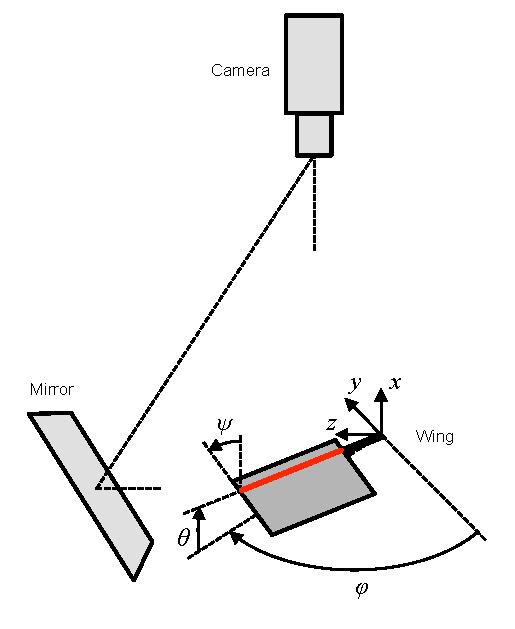
\includegraphics[trim=0 15 0 5, clip, width=0.5\textwidth]{figures/apparatus}
\caption{Schematic diagram of the experimental apparatus
  showing three kinematic variables of the wing motion: Stroke ($\phi$),
  deflection ($\psi$) and deviation ($\theta$).\label{fig:apparatus}}
\end{figure}


\subsection*{3D Printed wings and actuation mechanism}
The experimental wings were fabricated using an Objet Connex500 3D printer with
the rigid Objet FullCure720 material. In prior work, we demonstrated flapping
flight of a micro air vehicle with wings made using this material
\cite{richter2011untethered}. The wing design consisted of an interlocking
hinged root and tip, allowing the wing surface to pivot naturally during
flapping from its neutral vertical position to a deflection angle of
approximately 45\textdegree.  The wing design is illustrated in
Figure~\ref{fig:wing1} and the hinge design is illustrated in
Figure~\ref{fig:root2}.  In total, eleven wings were used, ranging in wingspan
from 40 mm to 120 mm and ranging in chord length from 40 mm to 80 mm. Flapping
amplitudes were constrained by the geometry of the wing root design to be set at
72\textdegree, 81\textdegree, and 96\textdegree, and each wing was flapped at
speeds ranging between 1 Hz and 3.5 Hz for each of these amplitude settings.  68
sets of data were recorded, representing Reynolds numbers between 2500 and 5000.

% See https://tex.stackexchange.com/questions/286737/sub-figures-of-different-sizes-grid-layout
\begin{figure}[h]%[!htb]
\centering
\begin{subfigure}[t]{0.45\textwidth}
    \centering
    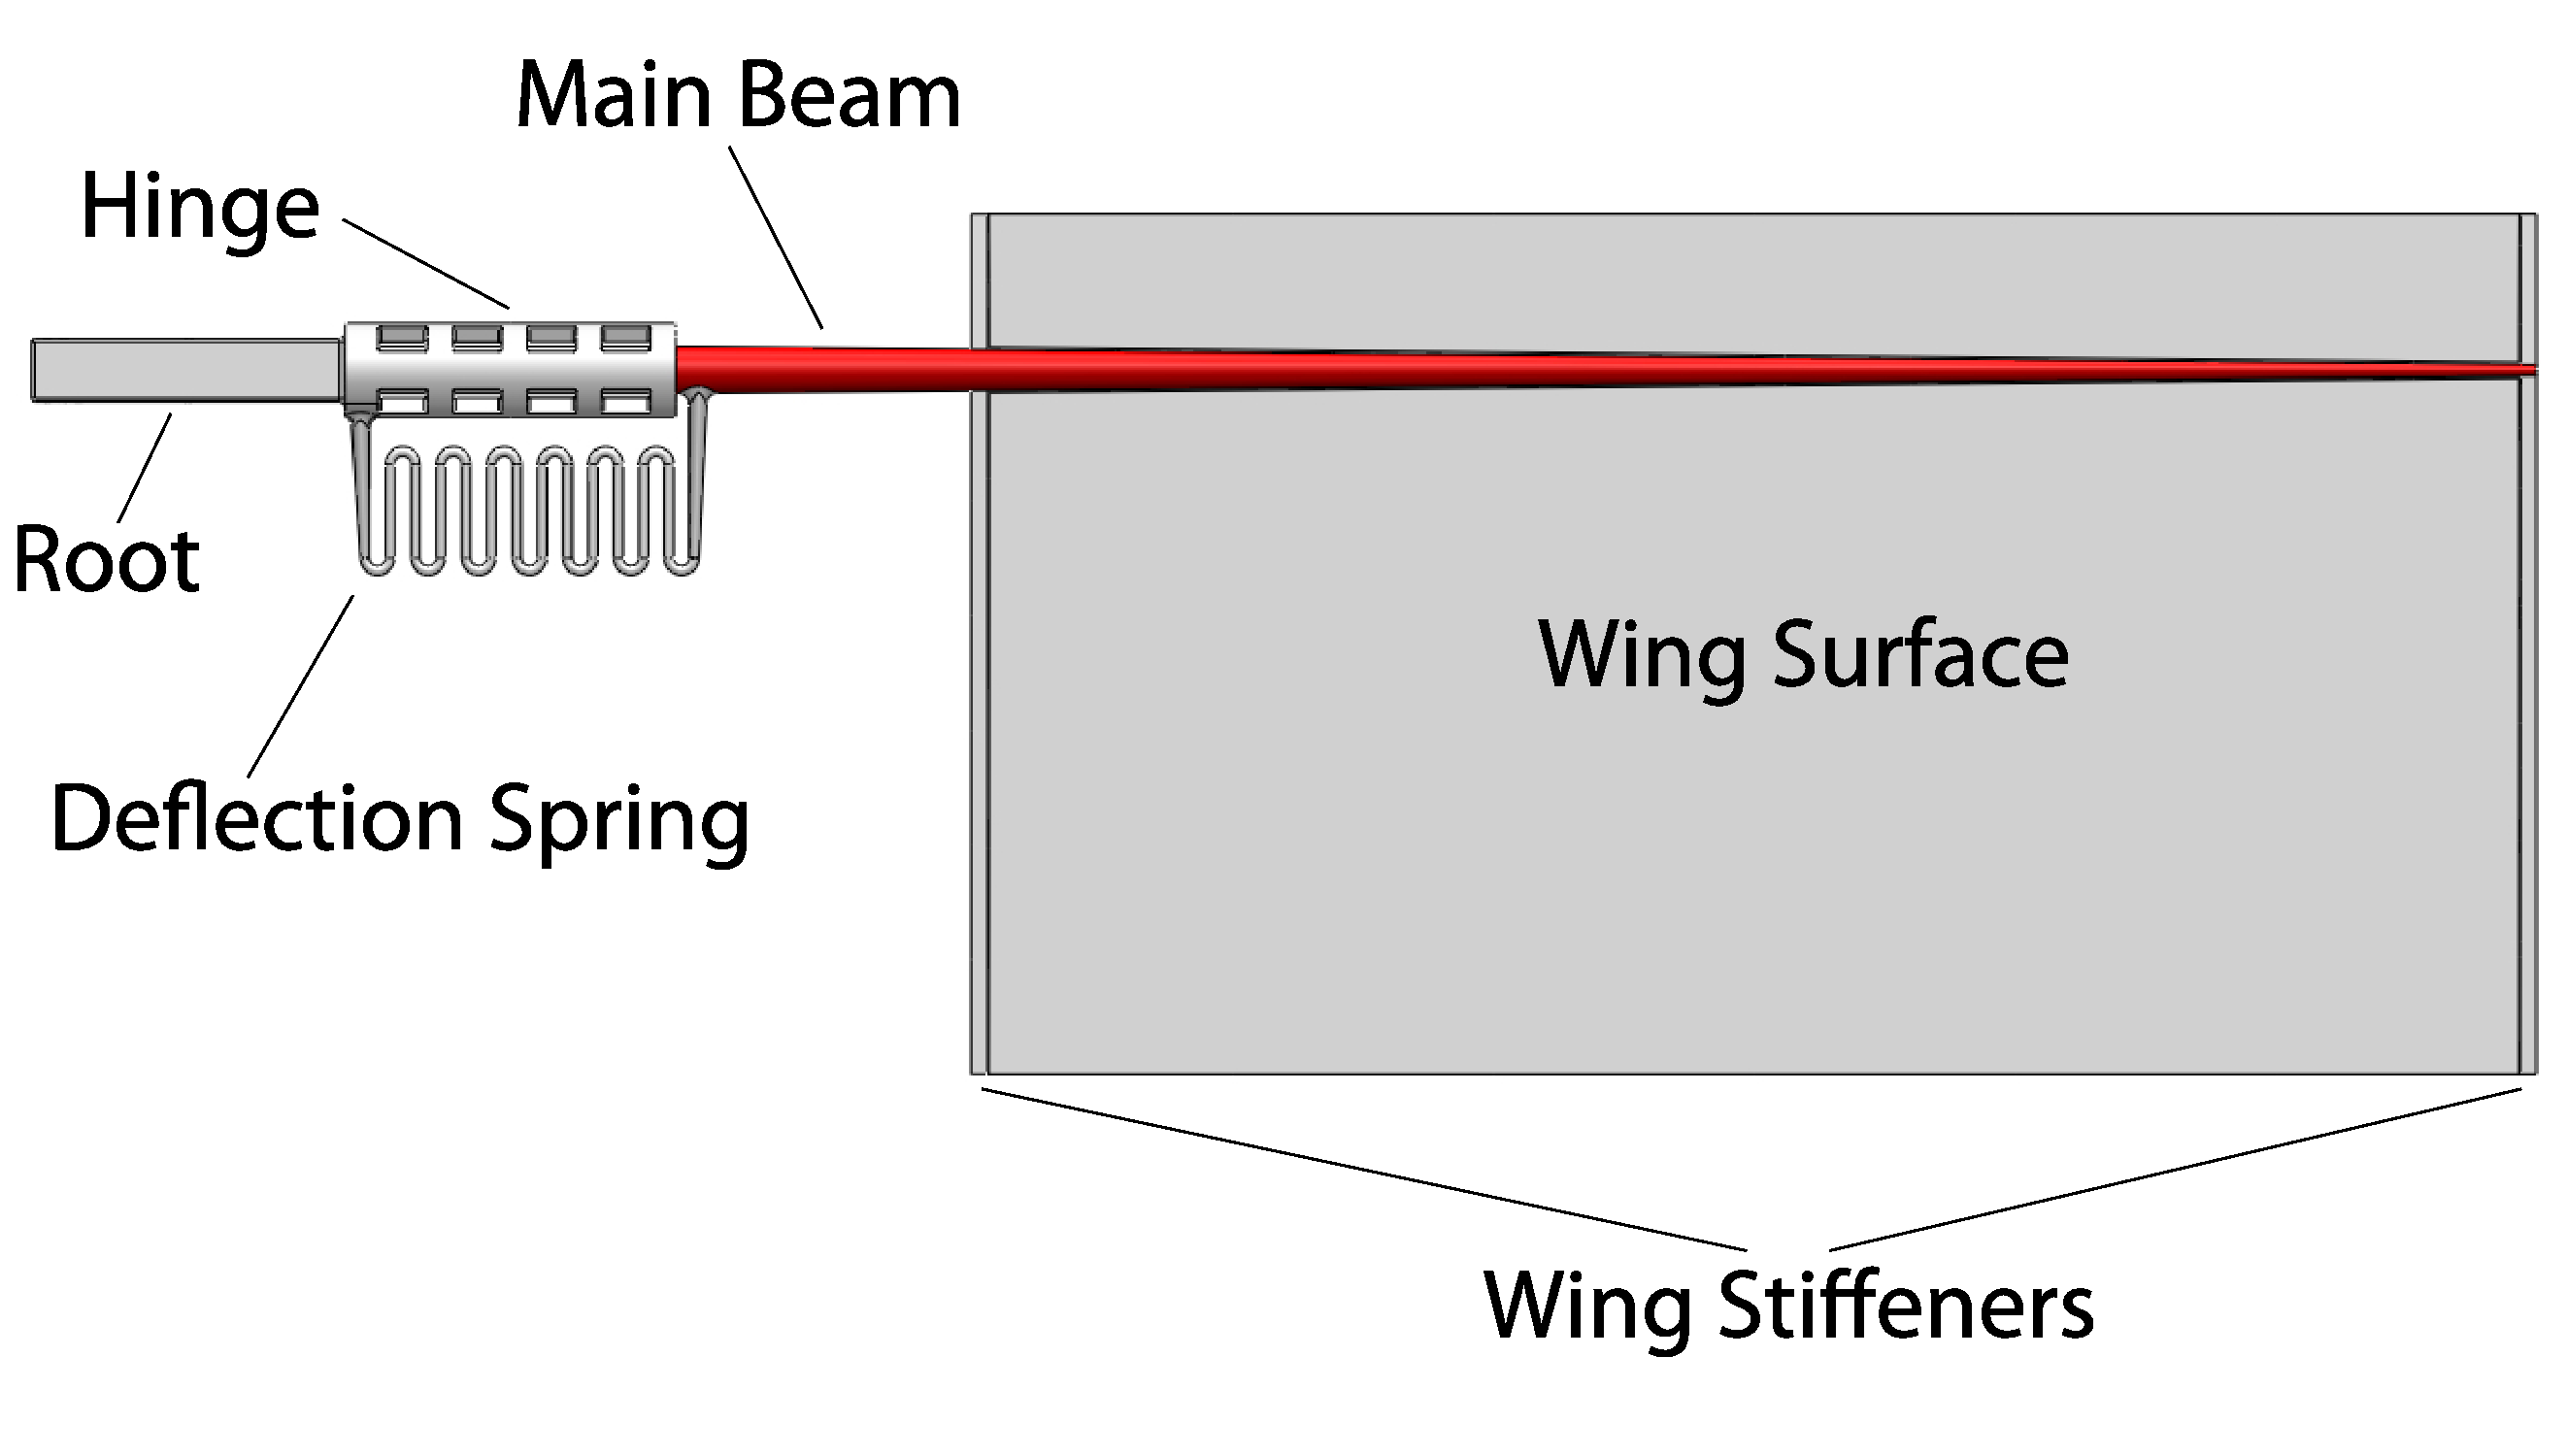
\includegraphics[width=0.95\textwidth]{figures/wing1}
    \caption{\label{fig:wing1}}
\end{subfigure}
\begin{subfigure}[t]{0.45\textwidth}
    \centering
    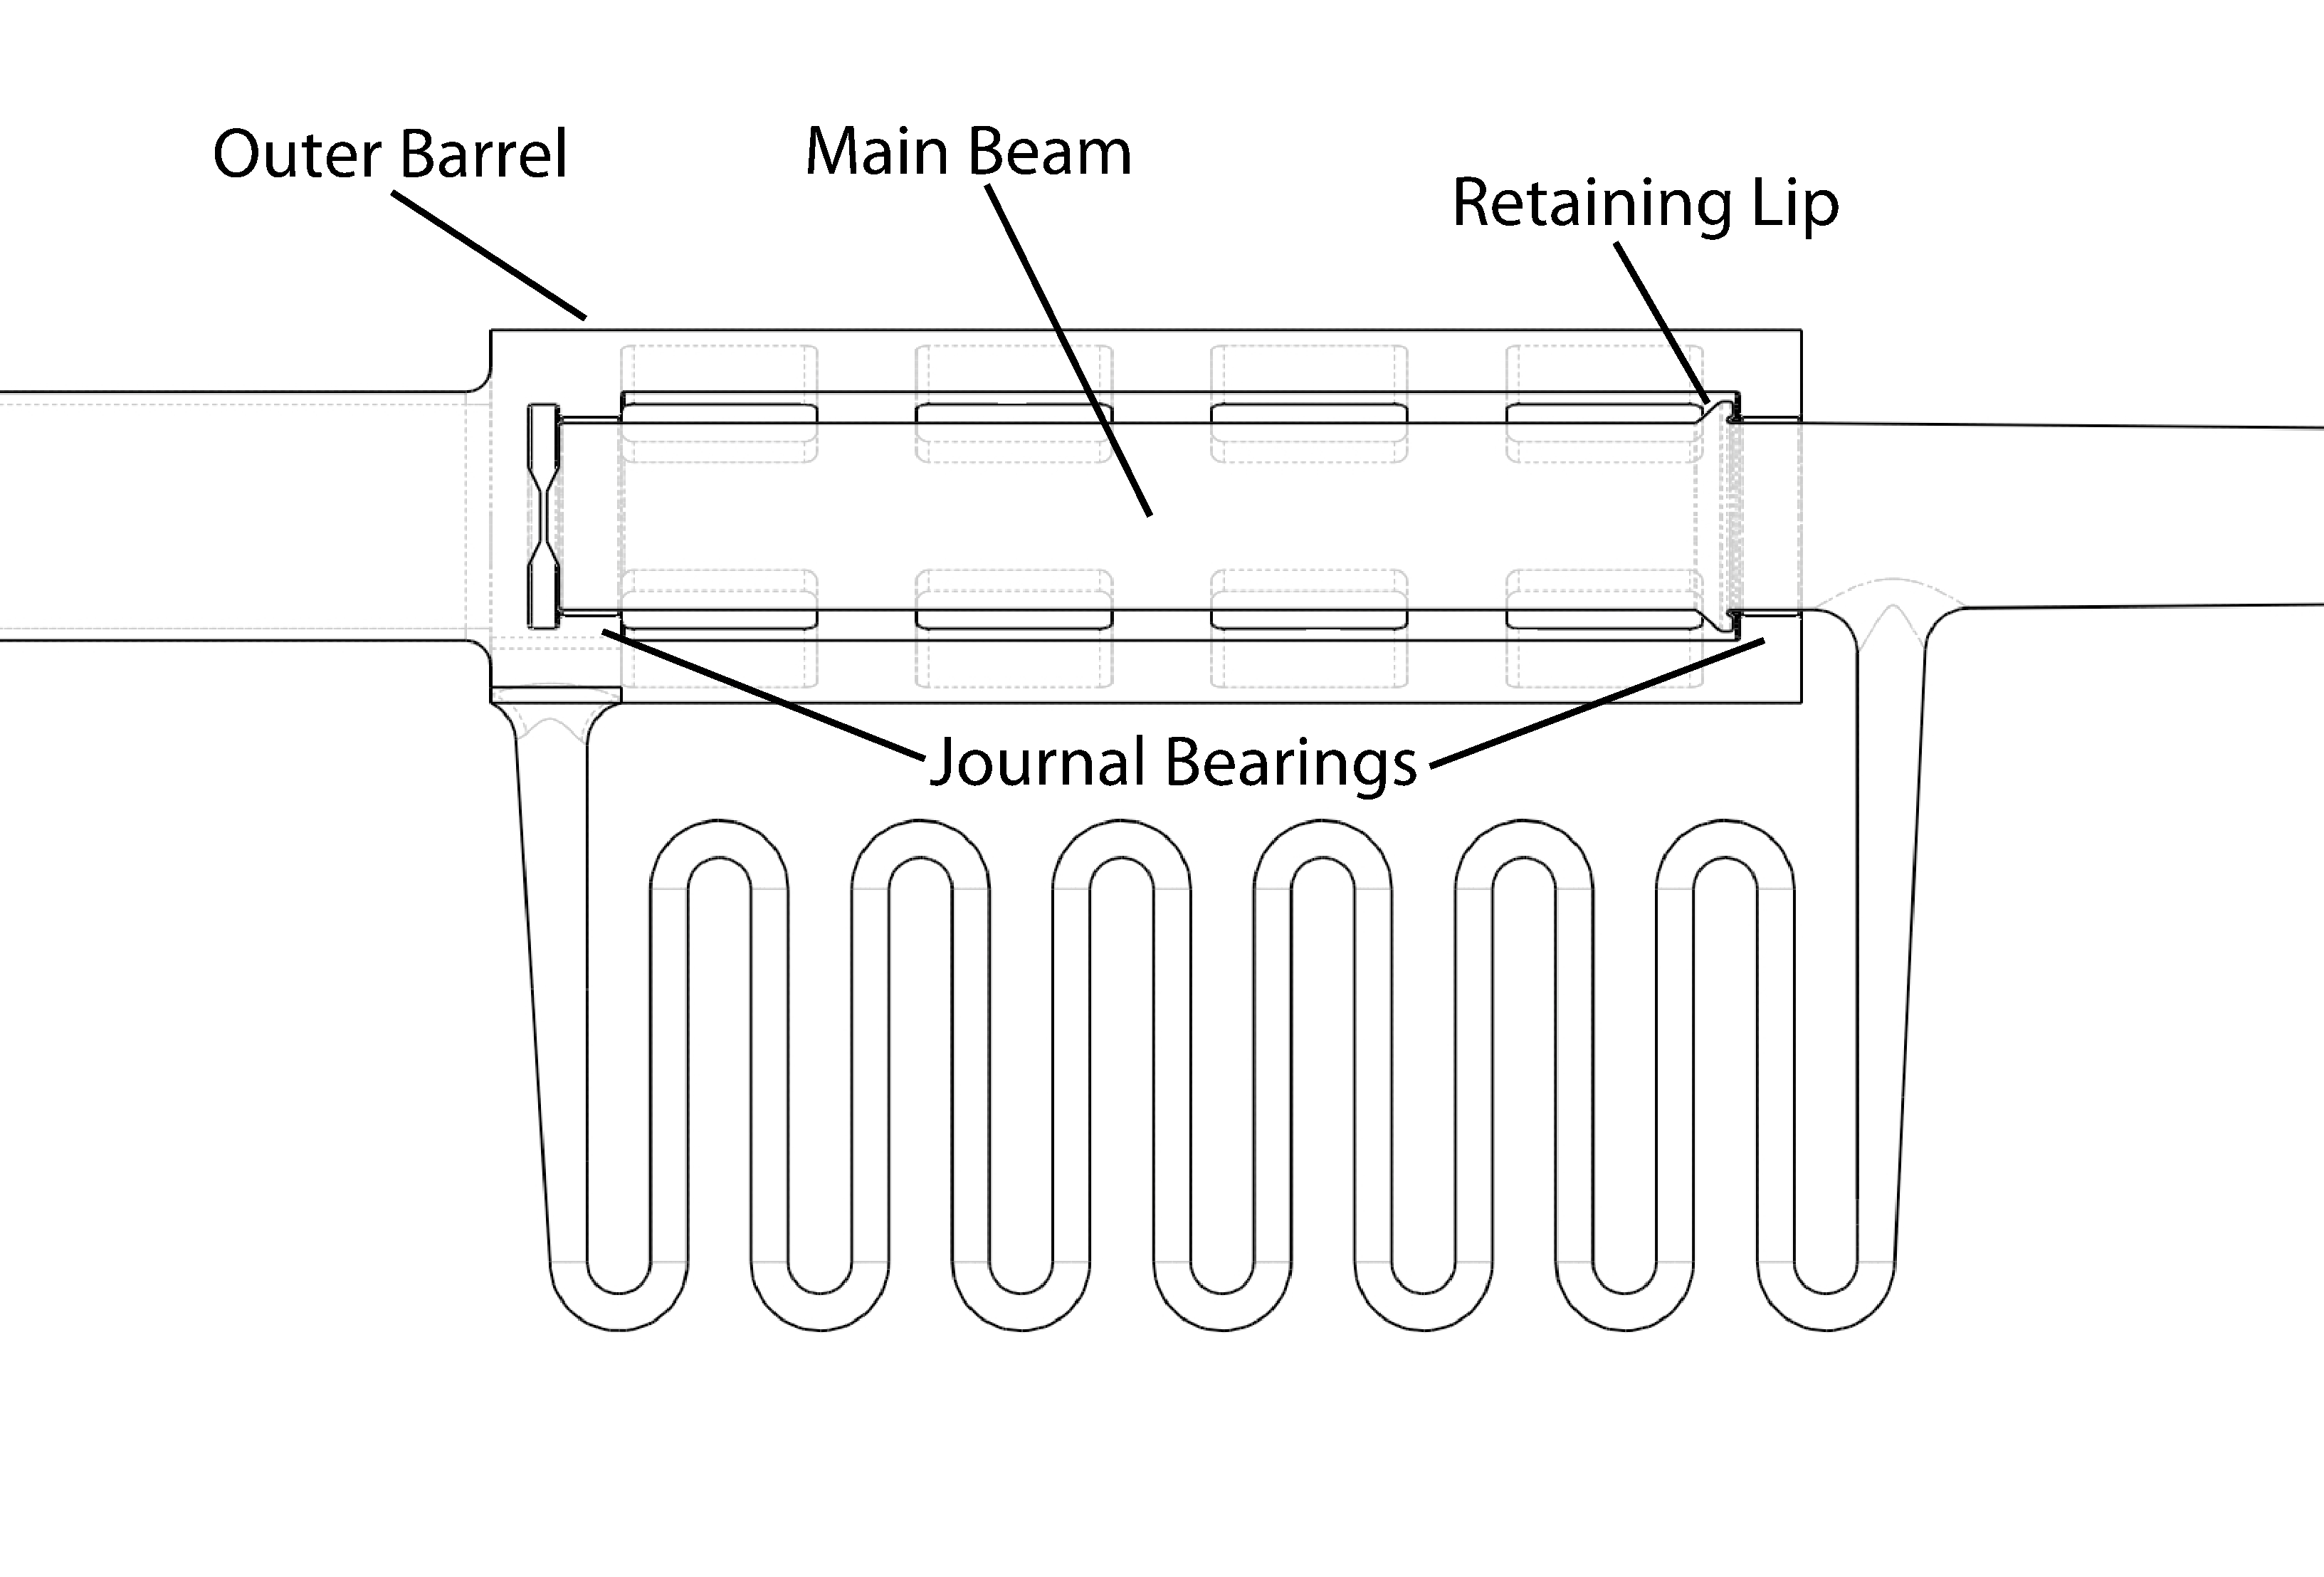
\includegraphics[trim=0 105 0 0, clip, width=0.95\textwidth]{figures/root2}
    \caption{\label{fig:root2}}
\end{subfigure}
\caption{Detail of 3D printed wing \subref{fig:wing1} and wing root \subref{fig:root2} design
  showing concentric-cylindrical design to allow passive pivoting of the wing surface.}
\end{figure}

\subsection*{Measurement apparatus}
The force measurement apparatus was based on a FUTEK LSM250 parallelogram load
cell, capable of a sampling rate of 1 kHz and a precision of 1\e{-9} N.  Mounted
directly to the load cell was a wing-flapping mechanism, which consisted of a DC
gear motor powering a crank and connecting rod used to drive the experimental
wings in a roughly sinusoidal flapping motion. This system is pictured in
Figures~\ref{fig:apparatus2} and \ref{fig:apparatus3}.  The natural vibration
frequency of the load cell and wing driving mechanism was roughly 70 Hz, the
natural vibration frequency for the first bending mode of the experimental wing
was approximately 26 Hz, and experimental wings were flapped at or below
approximately 3.5 Hz.  All experimental force measurements were filtered using a
high-order zero-phase digital low-pass filter with a cutoff frequency of 7.5
times the flapping frequency, which preserved the primary inertial and
aerodynamic forces acting on the wings while eliminating the faster vibrations
of the wing structure and the load cell apparatus.

% TODO: Mention empirically measuring impulse response.

% See https://tex.stackexchange.com/questions/286737/sub-figures-of-different-sizes-grid-layout
\begin{figure}%[!htb]
\centering
\begin{subfigure}[t]{0.45\textwidth}
    \centering
    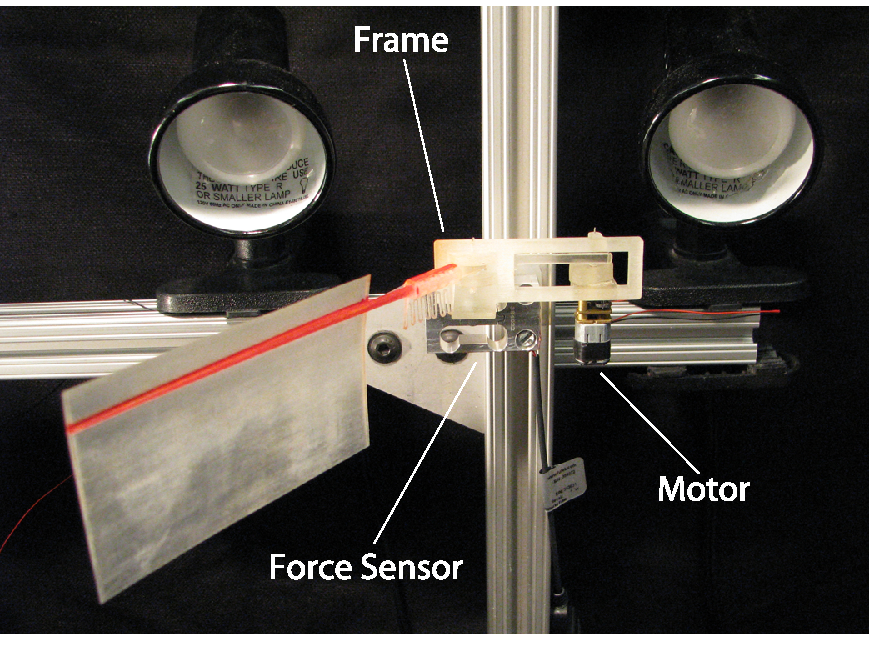
\includegraphics[height=5cm]{figures/apparatus2}
    \caption{\label{fig:apparatus2}}
\end{subfigure}
\begin{subfigure}[t]{0.45\textwidth}
    \centering
    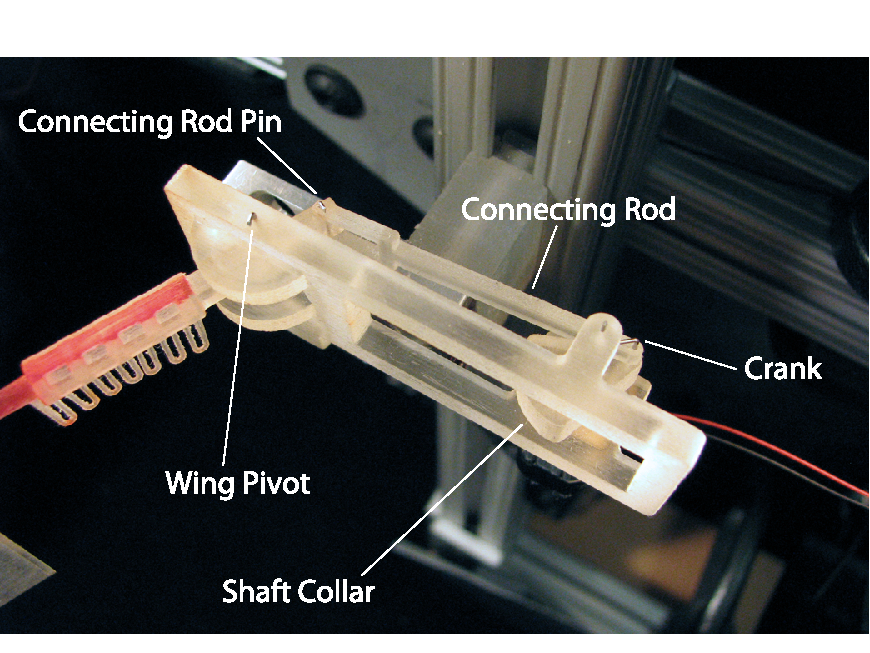
\includegraphics[height=5cm]{figures/apparatus3}
    \caption{\label{fig:apparatus3}}
\end{subfigure}
\caption{\subref{fig:apparatus2} Front view of the flapping wing apparatus
  showing the wing mounted on its driving mechanism attached to the force
  sensor. \subref{fig:apparatus3} Close-up view of the 3D printed frame and
  crank mechanism used to drive the flapping motion of the wing.}
\end{figure}

\subsection*{High-speed measurement of flapping kinematics}
A Casio EXILIM EX-FH20 color video camera was used to record each experiment at
210 frames per second from a top-down perspective as well as a side view
provided by a mirror mounted in the field of view. Both the top-down and side
views featured matte black backdrops to facilitate easy identification of the
wing in video frames. A variety of image-processing techniques were used to
extract the kinematics of the wing motion from each video frame. The main beam
of each wing was colored red and identified with a color filter in the top-down
view. A line was then fitted using the Hough Transform to identify the stroke
angle. The wing deflection angle was computed by measuring the projected area of
the wing in the top-down view, calibrated using the known dimensions of the
rectangular wing shape. The out-of-plane deviation angle of the wing was
measured by tracking the leading and trailing edge corners of the wingtip in the
side view and comparing their positions to the nominal position of the wingtip
with zero deflection and deviation throughout the wing stroke. We refer the
reader to our previous work for further details and illustrations of our methods
for extracting wing kinematics from high speed video and processing the measured
data~\cite{richter2012thesis}.

\subsection*{Data Smoothing and Registration}
Stroke, deflection and deviation measurements were smoothed with a
Savitzky–Golay filter, providing not only a reduction in noise in the signals
themselves, but also smooth first and second derivatives of these signals. These
kinematic variables were temporally aligned and resampled to the 1 kHz frequency
of the force measurement. Finally, for each wing at each flapping frequency and
amplitude, the data for 10-20 wing strokes were registered and averaged together
to create a composite sample representing the force and kinematics of a single
complete wing stroke of the given wing, frequency and amplitude. These composite
samples were then used for data-driven modeling and analysis.

% TODO: Mention polynomial fitting then differentiation to get derivatives.

% Figure~\ref{fig:kinematics} provides sample force data and measured wing
% kinematics from one experiment.


% \begin{figure}[ht]
% \centering
% 
\includegraphics[width=\linewidth]{figures/stream}
% \caption{Legend (350 words max). Example legend text.}
% \label{fig:stream}
% \end{figure}

% \begin{figure}
% \centering
% \begin{subfigure}[b]{.45\linewidth}
% 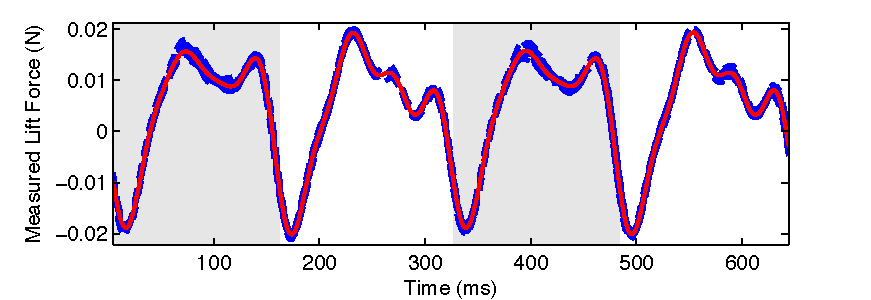
\includegraphics[width=\linewidth]{figures/regforce1}
% \caption{Measured vertical force.}
% \label{fig:regforce}
% \end{subfigure}
% \begin{subfigure}[b]{.45\linewidth}
% 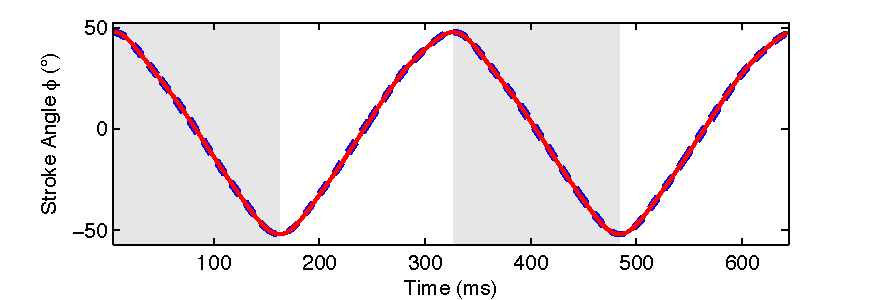
\includegraphics[width=\linewidth]{figures/regstroke1}
% \caption{Wing stroke angle.}
% \label{fig:regstroke}
% \end{subfigure}

% \begin{subfigure}[b]{.45\linewidth}
% 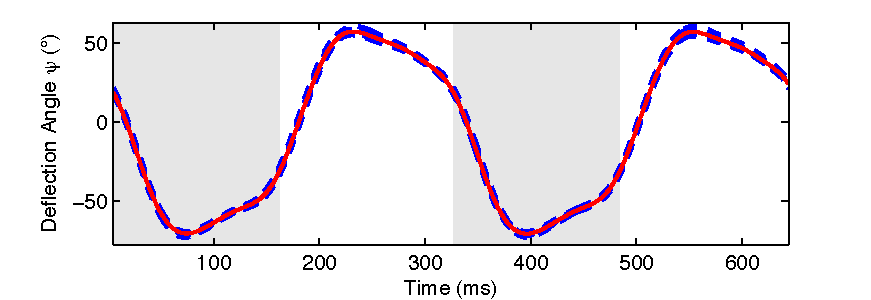
\includegraphics[width=\linewidth]{figures/regdef1}
% \caption{Wing deflection angle.}
% \label{fig:regdef}
% \end{subfigure}
% \begin{subfigure}[b]{.45\linewidth}
% 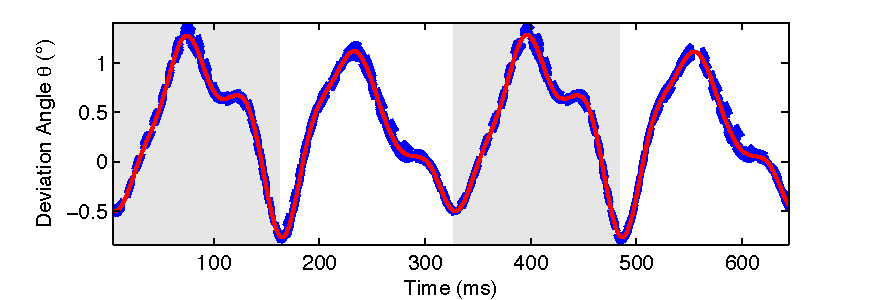
\includegraphics[width=\linewidth]{figures/regdev1}
% \caption{Wing deviation angle.}
% \label{fig:regdev}
% \end{subfigure}
% \caption{Measured \subref{fig:regforce} vertical force, \subref{fig:regstroke} wing stroke angle,
%   \subref{fig:regdef} deflection angle, \subref{fig:regdev} and deviation angle from one experiment,
%   registered and averaged over 18 flapping periods.}
% \label{fig:kinematics}
% \end{figure}

\section*{Results}

% Up to three levels of \textbf{subheading} are permitted. Subheadings should not be numbered.
%
% \subsection*{Subsection}
%
% Example text under a subsection. Bulleted lists may be used where appropriate, e.g.
%
% \begin{itemize}
% \item First item
% \item Second item
% \end{itemize}
%
% \subsubsection*{Third-level section}
%  
% Topical subheadings are allowed.

% TODO: Reword this section to not focus on the number 58 right off the bat.
\subsection*{Data-driven models}
We trained a set of data-driven models to predict the instantaneous vertical
force produced by flapping wings as a function of the kinematic variables and
derivatives describing their motion, and geometric parameters describing the
wing shape, totaling 31 separate variables. We trained these models on data from
58 experiments, selected at random from our 68 total experiments, which
represent a diverse sampling of wing geometry, flapping speed and amplitude
combinations. The remaining 10 experiments were reserved for testing. Models
were trained using the symbolic regression algorithm developed by Schmidt and
Lipson \cite{schmidt2009distilling} to minimized the mean absolute error (MAE)
between measured and predicted vertical force. The training process ran for
approximately 24 hours using 60 cores on a computing cluster.

By training on data representing a range of wing shapes and flapping speeds and
amplitudes, the model search effectively narrowed the large set of input
variables to the most preditive information and only utilized those terms that
accounted for variations in kinematics and wing geometry between experiments.
Table~\ref{table:eqmodels} lists the performance of five of the leading
candidate models, along with five analytical models for comparison, as measured
by MAE in the 10 test set experiments withheld from training. These five models
were selected from the Pareto frontier between MAE and formula complexity when
training was terminated. The data-driven models presented here are functions of
the kinematic variables ($\phi$, $\psi$, and $\theta$) and their derivatives,
the wing span ($R$), the span-wise and chord-wise locations of the center of
wing area ($X_{CM}$ and $Y_{CM}$), and constant coefficients. The analytical
models for comparison will be described in the following section.

Our primary results, provided in the column labeled ``MAE Not Fitted'', use
fixed coefficient values for all models that were jointly optimized on the
training set.  However, since the accuracy of the analytical models may depend
on coefficients that vary with wing shape, flapping speed, or other factors, we
also provide secondary results in the column labeled ``MAE Fitted'', which use
coefficient values that were fitted individually to each of the test set
experiments. In both categories of results, the data-driven models are more
accurate, demonstrating that the relative performance of data-driven models is
not simply due to the choice or optimization of coefficient values.

% TODO: Make sure to define all variables used in these tables.
% TODO: Figure out why we're calling it "U-squared". -->> Change to V^2
% everywhere (see Whitney Wood paper just below equation 2.18).
% TODO: If U-squared is "velocity squared" then  make sure that's consistent
% with the use of $v^2$ in the L_{trans} formula (equation 1) and elsewhere.
% TODO: Decide on better terms than "fitted" and "not fitted".
% TODO: Explain that the 5 EQ models were taken from the Pareto frontier of
% complexity vs. accuracy at the time of convergence.
% TODO: Explain that C_1,...,C_5 are not the same in each EQ. Maybe do C_i,_j
\begin{table}[ht]
\small
\centering
\begin{tabular}{|l|l|r|r|r|}
\hline
  {\bf Model} & {\bf Terms/Formula} & {\bf Size} & \begin{tabular}{@{}c@{}}{\bf MAE (N)} \\
    Fitted\end{tabular} & \begin{tabular}{@{}c@{}}{\bf MAE (N)} \\ Not Fitted\end{tabular}\\
\hline
\(EQ _5\) & \(C_1RY_{CM}\dot{\psi}^2\ + C_2RX_{CM}\dot{\phi}\psi - C_3R\ddot{\theta}\) & 12 & 8.79\e{-4} & 1.19\e{-3}\\
\(EQ _4\) & \(C_1RY_{CM}\dot{\psi}^2\cos\psi + C_2RX_{CM}\dot{\phi}\psi - C_3R\ddot{\theta}\) & 14 & 8.66\e{-4} & 1.18\e{-3}\\
\(EQ _3\) & \(C_1RY_{CM}\dot{\psi}^2\cos(\psi-\psi^2) + C_2RX_{CM}\dot{\phi}\psi - C_3R\ddot{\theta}\) & 16 & 8.49\e{-4} & 1.14\e{-3}\\
\(EQ _2\) & \(C_1RY_{CM}\dot{\psi}^2\cos\psi + C_2RX_{CM}\dot{\phi}\psi - C_3R\dot{\phi}\dot{\psi}\psi - C_4R\ddot{\theta}\) & 19 & 8.15\e{-4} & 1.14\e{-3}\\
\(EQ _1\) & \(C_1RY_{CM}\dot{\psi}^2\cos\psi + C_2RX_{CM}\dot{\phi}\psi - C_3R\ddot{\theta}\dot{\phi}\psi - C_4R\dot{\phi}\dot{\psi}\psi - C_5R\ddot{\theta}\) & 24 & 7.73\e{-4} & 1.12\e{-3}\\
\hline
\(V^2\) Planar 1 & \(L_{planar},  F_{pendulum}\) & 32 & 1.38\e{-3} & 1.47\e{-3}\\
\(V^2\) Planar 2 & \(L_{planar}, F_{pendulum}, F_{deviation}\) & 46 & 1.18\e{-3} & 1.29\e{-3}\\
\(V^2\) Total & \(L_{trans}, F_{pendulum}, F_{deviation}\) & 96 & 1.18\e{-3} & 1.29\e{-3}\\
WW~\cite{whitney2010aeromechanics} & \(L_{trans}, AM_{trans}, AM_{rot}, F_{pendulum}, F_{deviation}\) & 121 & 1.02\e{-3} & 1.23\e{-3}\\
PW~\cite{pesavento2004falling} & \(L_{trans}, L_{rot}, AM_{trans},
    AM_{trans-rot}, F_{pendulum}, F_{deviation}\) & 130 & 1.01\e{-3} & 1.20\e{-3}\\
\hline
\end{tabular}
\caption{\label{table:eqmodels}Comparison of data-driven models and analytical
  equations of lift.  The models are sorted by equation size, which is
  calculated as the sum of arithmetic and trigonometric operators required to
  compute a force prediction from kinematic and geometric data.  MAE reports
  average mean absolute error (in Newtons of vertical force) for the ten test
  experiments.}
\end{table}

% TODO: Remove these:
% Analytical models for publication
% mean_nofit_mae_plpi =    1.4681e-03
% mean_nofit_mae_plti =    1.2881e-03
% mean_nofit_mae_rw_liftonly =    1.2870e-03
% mean_nofit_mae_rw_liftam =    1.2281e-03
% mean_nofit_mae_jw =    1.1985e-03
% Eureqa models
% mean_nofit_mae_eq1 =    1.1153e-03
% mean_nofit_mae_eq2 =    1.1429e-03
% mean_nofit_mae_eq3 =    1.1443e-03
% mean_nofit_mae_eq4 =    1.1769e-03
% mean_nofit_mae_eq6 =    1.1909e-03
% Fitting and testing on testing data...
% Analytical models for publication
% mean_fit_mae_plpi =    1.3793e-03
% mean_fit_mae_plti =    1.1836e-03
% mean_fit_mae_rw_liftonly =    1.1833e-03
% mean_fit_mae_rw_liftam =    1.0204e-03
% mean_fit_mae_jw =    1.0088e-03
% Eureqa models
% mean_fit_mae_eq1 =    7.7317e-04
% mean_fit_mae_eq2 =    8.1508e-04
% mean_fit_mae_eq3 =    8.4913e-04
% mean_fit_mae_eq4 =    8.6626e-04
% mean_fit_mae_eq6 =    8.7928e-04

\subsection*{Analytical models for comparison}
The analytical models used for comparison are also listed in
Table~\ref{table:eqmodels}.  These models consist of calculated inertial forces
added to a collection of aerodynamic terms.  The primary aerodynamic
contribution in all quasi-steady models is a translational lift term
proportional to the squared velocity of each span-element of the wing that is
related to the wing's angle of attack and empirically determined coefficient of
lift.  This term is labeled $L_{planar}$ when wing motions out of the nominal
horizontal flapping plane are neglected in the calculations, or $L_{trans}$ when
out-of-plane motions are included. This translational lift term is given by:
\begin{equation}
L_{trans}=(\nicefrac{1}{2})\rho V^2AC_L,
\end{equation}
where \(V\) is the wing velocity, \(\rho\) is the fluid density, \(A\) is the area of the wing surface, and \(C_L\) is the coefficient of lift.  The theoretical value of the coefficient of lift depends on the angle of attack \(\alpha\):
\begin{equation}
C_L = C_{Lmax}\sin(2\alpha).
\end{equation}
In Table~\ref{table:eqmodels} and Figure~\ref{fig:pareto_mae}, we present
results for three models whose only aerodynamic component is translational lift
proportional to wing velocity, which we term $V^2$ Planar 1, $V^2$ Planar 2, and
$V^2$ Total.

% TODO: Understand and verify (numerically) how we get an effective v^2 via
% integration along the span, and document that in the code.

Additional aerodynamic effects include rotational lift proportional to the
product of a wing's rotational and translational velocities, labeled $L_{rot}$,
as well as ``added-mass'' effects related to the accelerations of fluid
surrounding the wing \cite{sedov1965two}.  These added mass terms are
proportional to the wing's linear acceleration ($AM_{trans}$), rotational
acceleration ($AM_{rot}$), or a product of the two ($AM_{trans-rot}$). Whitney
and Wood~\cite{whitney2010aeromechanics} and Pesavento and
Wang~\cite{pesavento2004falling} describe quasi-steady models that use different
combinations of such terms. We refer to these models in
Table~\ref{table:eqmodels} and Figure~\ref{fig:pareto_mae} as WW and PW, respectively.

Inertial forces acting on the wings are modeled as a sum of two contributions.
The primary contribution results from the pendulum-like swinging motion that
occurs when the deflection angle ($\psi$) flips at stroke reversal.  The
secondary contribution results from small angle deviations from the horizontal
flapping plane ($\theta$). These inertial forces are given by:
\begin{equation}\label{sdbla}
F_{pendulum} = Y_{CM}M(\ddot{\psi}\sin\psi + \dot{\psi}^2\cos\psi)
\end{equation}
and
\begin{equation}\label{sdbla2}
F_{deviation} = -X_{CM}M(\ddot{\theta}\cos\theta - \dot{\theta}^2\sin\theta),
\end{equation}
\noindent where \(X_{CM}\) and \(Y_{CM}\) are the span-wise and chord-wise
locations of the center of wing area and \(M\) is the mass of the wing surface.
All of our analytical models for comparison include $F_{pendulum}$ and all
except $V^2$ Planar 1 include $F_{deviation}$.

% TODO: Remove all occurrences of the word "pareto" from the text, figures and filenames.
\begin{figure}
\centering
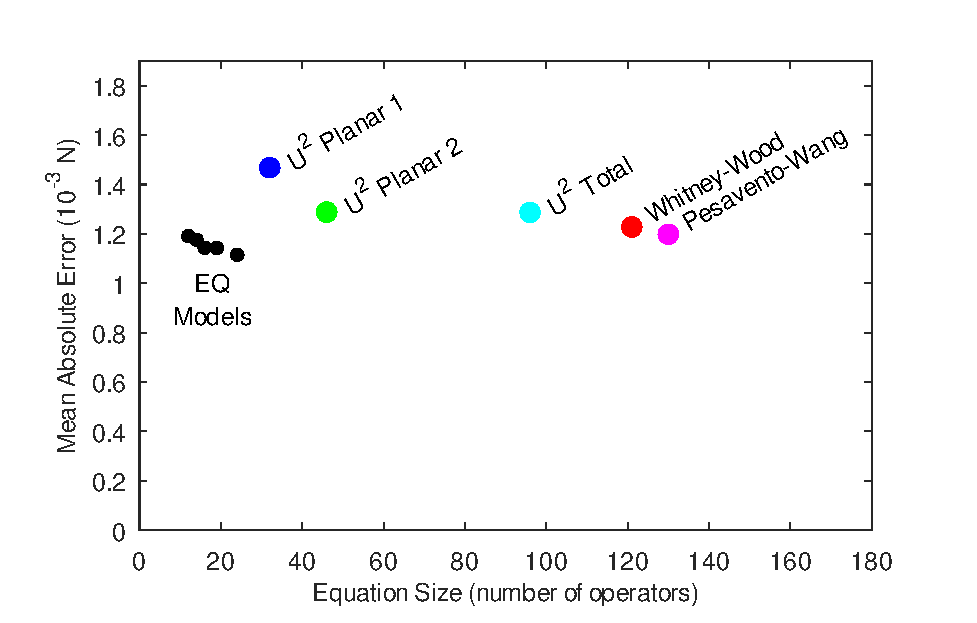
\includegraphics[width=0.5\textwidth]{figures/mae_nofit}
\caption{Pareto plot of all data-driven (``EQ Models'') and analytical models
  using mean values for model coefficients. All data-driven models were smaller
  and more accurate than analytical models.\label{fig:pareto_mae}}
\end{figure}

\subsection*{Evaluation of Model Performance}
An evaluation of model performance allows comparison between analytical models
and the equations developed through the data mining process.  Equations are
judged by their accuracy and complexity.  In this case, the complexity or size
of an equation was measured by simply counting the number of arithmetic and
trigonometric operators used to combine the measured kinematic variables and
geometric properties into an equation for instantaneous vertical force.  Both
our data-driven models and the analytical equations are measured in this way.
For fairness, constants in the analytical models that would have been lumped
together into larger coefficients by the symbolic regression algorithm (such as
material density, air density, \(\pi\) or factors of integration) are also
lumped together in the calculations of size for the analytical equations. The
size of the inertial calculations was added to the sizes of analytical lift
calculations.  The pendulum motion has an equation size of 13 and the total
inertial calculation including out-of-plane deviation has a size of 27.

Table~\ref{table:eqmodels} shows the size of all equations considered in this
study, and indicates that the analytical models are all significantly more
complex than our data-driven models.  One of the reasons for high complexity in
the analytical models is the dependence on wing geometry and integration of
forces over the span and chord of the wing.  A second reason for the complexity
in analytical models is the number of geometric and coordinate transformations
required to compute the necessary linear and rotational velocities.  In this
sense, several terms generated during symbolic regression can be considered to
be approximations of much more subtle calculations of kinematic quantities.

The accuracy of each equation was measured as the mean absolute error (MAE)
between the predicted and actual vertical force (in Newtons) produced by the
flapping wing.  Figure~\ref{fig:pareto_mae} shows the Pareto plot of all models
considered, depicting accuracy as a function of model complexity. It is
important to note that all data-driven models have between three and five
coefficients, so tuning these coefficients allows further minimization of error
compared to the analytical models, which have between one and three.
Nevertheless, discovery of models with smaller error than theoretical
predictions that are simultaneously much simpler is a significant feat for the
data mining process and symbolic regression.

\begin{figure}[ht]
\centering
\begin{tabular}{cc}
\begin{subfigure}{0.48\textwidth}
\centering
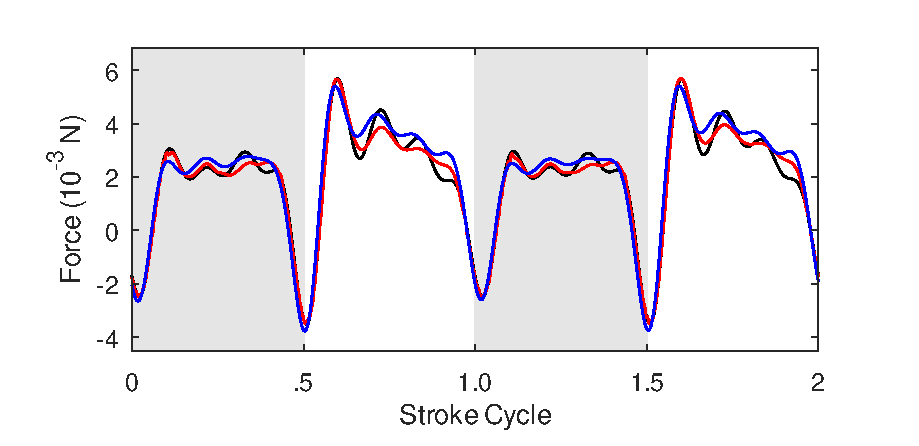
\includegraphics[width=\textwidth]{figures/eq_goodbad_1}
\caption{\label{fig:eq_goodbad_1} Training data.}
\end{subfigure} &
\begin{subfigure}{0.48\textwidth}
\centering
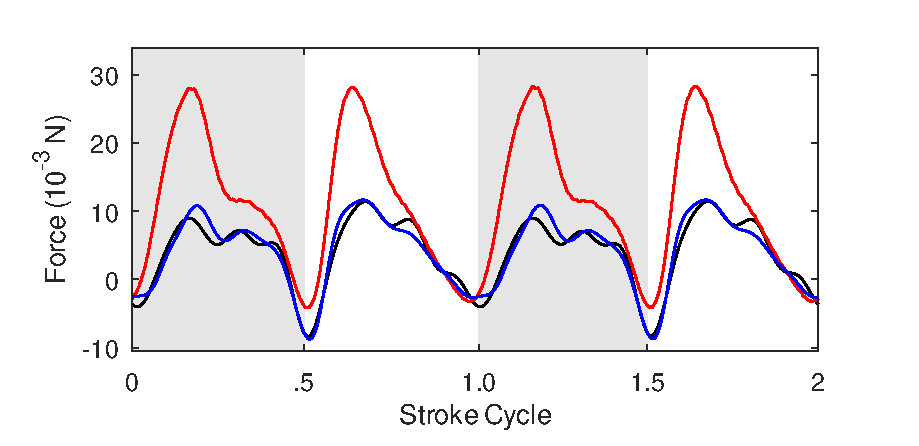
\includegraphics[width=\textwidth]{figures/eq_goodbad_2}
\caption{\label{fig:eq_goodbad_2} Test data \#1.}
\end{subfigure} \\
\begin{subfigure}{0.48\textwidth}
\centering
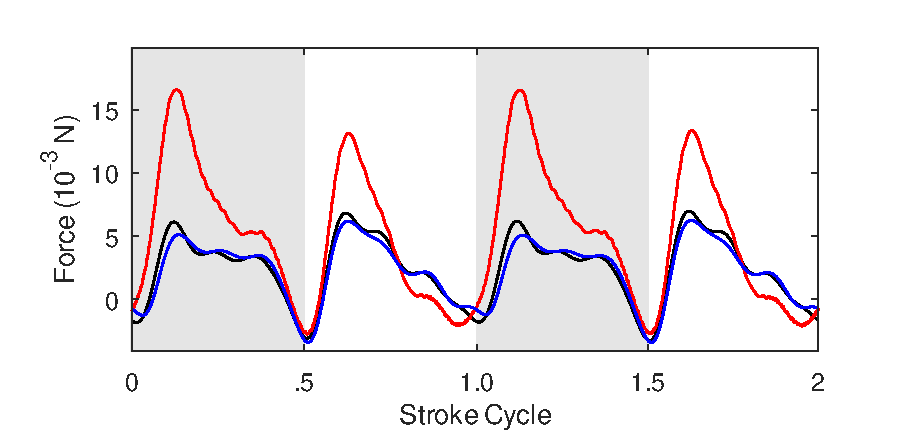
\includegraphics[width=\textwidth]{figures/eq_goodbad_3}
\caption{\label{fig:eq_goodbad_3} Test data \#2.}
\end{subfigure} &
\begin{subfigure}{0.48\textwidth}
\centering
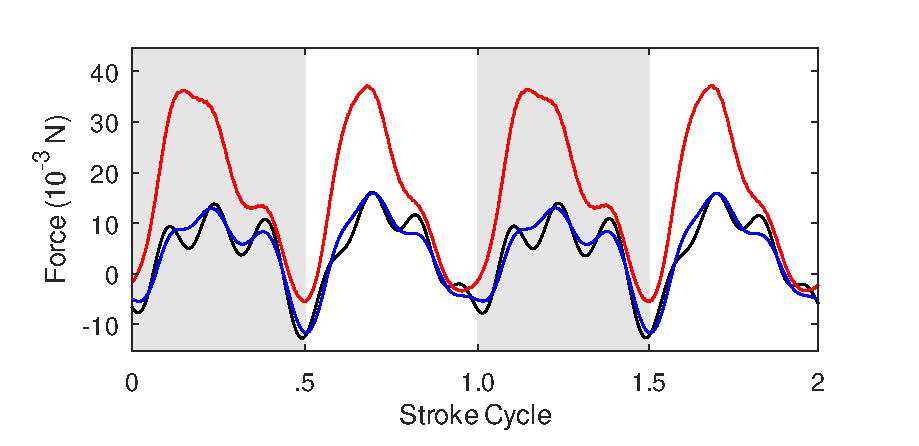
\includegraphics[width=\textwidth]{figures/eq_goodbad_4}
\caption{\label{fig:eq_goodbad_4} Test data \#3.}
\end{subfigure}
\end{tabular}
\caption{Comparison of force predictions between $EQ_4$ (blue) and
Equation~\eqref{eq:badeq} (red). $EQ_4$ was trained on 58 distinct experiments
simultaneously, including the data shown in~\subref{fig:eq_goodbad_1}, whereas
Equation~\eqref{eq:badeq} was trained \emph{only} on the data shown
in~\subref{fig:eq_goodbad_1}.  \subref{fig:eq_goodbad_1} shows that both models
perform well on this data within their training sets.  However, when presented
with test data \subref{fig:eq_goodbad_2}, \subref{fig:eq_goodbad_3} and
\subref{fig:eq_goodbad_4} not contained within either model's training set, only $EQ_4$ is able to
generalize and provide accurate predictions, while Equation~\eqref{eq:badeq}
fails to do so.}
\label{fig:eq_goodbad}
\end{figure}

\subsection*{Performance of models trained on one experiment versus many experiments}
Figure~\ref{fig:eq_goodbad_1} illustrates the predictive performance of two
models on data within their training sets, while
Figures~\ref{fig:eq_goodbad_2},~\ref{fig:eq_goodbad_3},
and~\ref{fig:eq_goodbad_4} illustrate the performance of those same two models
on data outside their training sets. The differences between these two models
result from the fact that one of them, $EQ_4$ from Table~\ref{table:eqmodels}
(drawn in blue), was trained on 58 separate experiments simultaneously, whereas
the other one, shown below (drawn in red), is one of many models trained only on
the single experiment shown in Figure~\ref{fig:eq_goodbad_1}:
\begin{align}
 Force = \frac{C_1 + C_2\psi^2 - C_3\psi}{C_4 + \ddot{\theta} + C_5\dot{\theta} + \cos(C_6 -
  \frac{C_7}{\psi^2} - C_8\psi)} - C_9.
\label{eq:badeq}
\end{align}
Thus, $EQ_4$ shows strong qualitative and quantitative agreement with all of the
experiments in Figure~\ref{fig:eq_goodbad}, indicating that this model is not
over-fit but in fact generalizes well to new data. Equation~\eqref{eq:badeq}, on
the other hand, fails to accurately predict the recorded data outside its
training set.  Insufficient data and over-fitting are potential pitfalls of
data-driven modeling, but are overcome in this case with a diverse sampling of
training data.

Since Equation~\eqref{eq:badeq} is unable to accurately predict forces outside
its training set, it is unlikely to offer any insight into the underlying
physical processes.  $EQ_4$, however, must capture some of the underlying
structure of the physics in order to generalize to data upon which it was not
trained.  In data-driven modeling, training on many experiments simultaneously
helps to reject candidate equations that may fit some, but not all, of the data,
and helps to retain those models that reflect the underlying physics and offer
insight into the structure of the additive components that compose the observed
behavior of a complex dynamical system.

\subsection*{Correspondence of physical terms}
One powerful result of the data-driven modeling approach is that in many cases,
certain terms from the data-driven models closely match physically
understandable terms from the analytical models.  The correspondence between
these terms is listed in Table~\ref{table:eqcorrespondence}. Taking model $EQ_4$
as an example, all three terms show strong resemblance to inertial and
aerodynamic components of the analytical models.  Figure~\ref{fig:eqcomparison}
shows a comparison between the simple velocity-squared aerodynamic lift
prediction and the second term of $EQ_4$: \(C_2RX_{CM}\psi\dot{\phi}\).  These
two calculations are numerically very similar, yet the third term of $EQ_4$ is
much simpler than $L_{trans}$.

Similarly, the sum of terms 1 and 3, \(C_1RY_{CM}\dot{\psi}^2\cos(\psi) -
C_3R\ddot{\theta}\), closely approximates the calculation of inertial forces
including the pendulum motion of the wing as well as the out-of-plane deviation.
Figure~\ref{fig:eqcomparison} also shows these two calculations, indicating very
similar structure.  While $EQ_4$'s approximation of these inertial forces does
not precisely match the analytical calculation, it follows a very similar
pattern and is much simpler.  Remarkably, these inertial terms utilize some of
the same variable combinations as the analytical calculations to express the
inertial force, namely \(Y_{CM}\dot{\psi}^2\cos(\psi)\) and \(\ddot{\theta}\),
with different coefficients to express the geometric variation between wings and
small angle approximations \(\cos\theta\approx1\), \(\sin\theta\approx0\) for
small out-of-plane deviation angles.  Since \(|\theta|<2^{\circ}\) in general,
the small angle approximation is valid.

\begin{table}[ht]
\centering
\begin{tabular}{|l|l|l|}
\hline
{\bf Contribution} & {\bf Analytical} & {\bf Data-Driven ($EQ_4$)}\\
\hline
Aerodynamic Lift & \(\nicefrac{1}{2}\rho v^2AC_{Lmax}\sin(2\alpha)\) & \(C_2RX_{CM}\psi\dot{\phi}\)\\
Pendulum 1 & \(M\cdot Y_{CM}\ddot{\psi}\sin{\psi}\) & \it{None} \\
Pendulum 2 & \(M\cdot Y_{CM}\dot{\psi}^2\cos{\psi}\) & \(C_1R\cdot Y_{CM}\dot{\psi}^2\cos{\psi}\) \\
Deviation 1 & \(\approx-MX_{CM}\ddot{\theta}\) & \(- C_3R\ddot{\theta}\)\\
Deviation 2 & \(\approx0\) & \it{None} \\
%Deviation 2 & \(X_{CM}M\dot{\theta}^2\sin\theta\) & \(<none>\)\\
\hline
\end{tabular}
\caption{\label{table:eqcorrespondence}Correspondence between analytical and data-driven terms.}
\end{table}

\begin{figure}[ht]
\centering
\begin{subfigure}{0.48\textwidth}
\centering
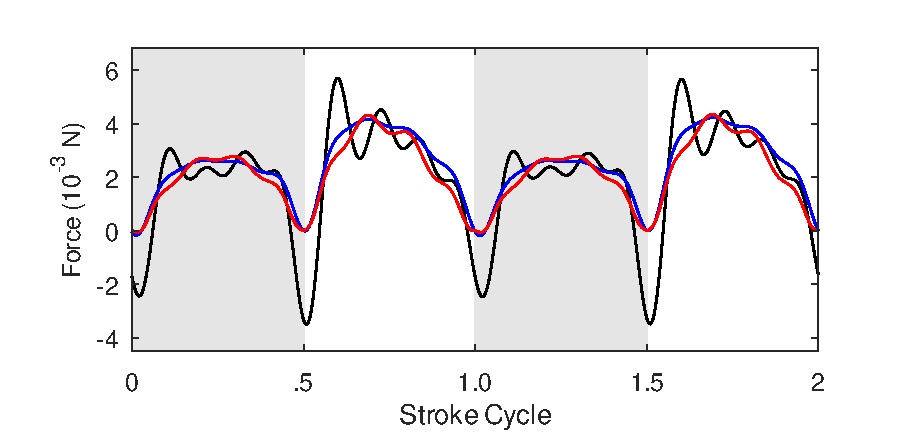
\includegraphics[width=\textwidth]{figures/eq_comparison_lift}
\caption{\label{fig:eqcomparison_lift} Aerodynamic lift forces.}
\end{subfigure}
% \qquad
\begin{subfigure}{0.48\textwidth}
\centering
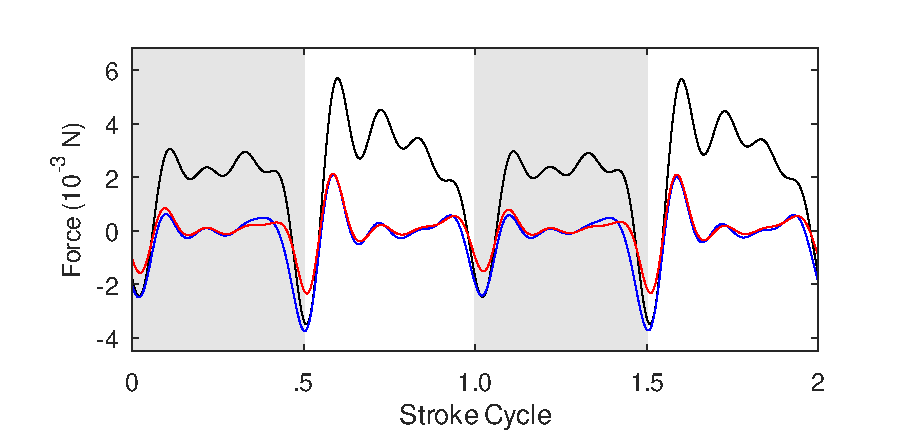
\includegraphics[width=\textwidth]{figures/eq_comparison_inertial}
\caption{\label{fig:eqcomparison_inertial} Inertial forces.}
\end{subfigure}
\caption{Comparison between terms of the analytical expressions (red) and
  data-driven models (blue).  \subref{fig:eqcomparison_lift} Primary
  translational aerodynamic lift proportional to the square of the wing
  velocity. \subref{fig:eqcomparison_inertial} Inertial forces related to the
  pendulum motion of the wing and deviation out of the stroke plane. The
  modeling process automatically decoupled aerodynamic and inertial effects with
  no prior knowledge of the system. The total measured force is shown for
  reference (black).}
\label{fig:eqcomparison}
\end{figure}

\section*{Discussion}

% The Discussion should be succinct and must not contain subheadings.

Table~\ref{table:eqcorrespondence} lists the corresponding terms between the
basic analytical expressions and the data-driven model $EQ_4$.  While two of the
inertial terms share the same combinations of variables, the data-driven
expression for aerodynamic lift is very different from its analytical
counterpart, and one portion of the pendulum motion is omitted altogether from
the data-driven models.  The reasons for these differences lie in the nature of
the symbolic regression algorithm, which is designed to return only the most
parsimonious expressions capable of predicting the experimental data at a given
level of accuracy.  Therefore, key physical effects may be represented
numerically by terms that are symbolically different and often much simpler than
their analytical counterparts.  This behavior of automatically separating
distinct dynamical building blocks is one of the most powerful aspects of
symbolic regression.  By sweeping the range of several kinematic and geometric
parameters in the 58 sets of training data, any candidate models that
incorrectly mix or couple two separate physical effects are discarded upon
testing on a data set with different parameters.  

Nevertheless, in some domains such as flapping flight, there exist high degrees
of correlation between certain variables.  For example, the center of area
location in a rectangular wing is closely related to its span and chord length.
Similarly, kinematic variables such as stroke and deflection angles are highly
correlated with each other and their derivatives across all 58 experiments,
making these variables approximately interchangeable with each other when
coefficients are adjusted accordingly.  This behavior provides an explanation
for why \(\psi\dot{\phi}\) is used as an approximation for an aerodynamic lift
term proportional to \(v^2\).  These correlations between variables are
inherent in highly symmetric, periodic phenomena such as flapping flight.  In
principle, additional experiments could be performed on flapping surfaces that
are not bound to the natural kinematics of flapping wings to explore the full
parameter space and disambiguate non-physical terms in the candidate models.

% \section{Conclusions} 
The major thrust of this work was to apply a data-driven approach to modeling
the forces on a flapping wing.  The models produced by our symbolic regression
algorithm were shown to be more accurate than any of the analytical models, and
were much simpler, in some cases by an order of magnitude in equation size.
Furthermore, by dissecting these equations and examining individual terms, it
was observed that the data-driven models separated the measured forces into
understandable physical effects.  A lift term was found that was numerically
similar to the standard translational lift, and an inertial term was found that
was numerically similar to the complete calculation of the pendulum and
out-of-plane motions with some analytical terms in common.  Finally, by training
data-driven models on experimental data from 58 individual wing-amplitude-speed
combinations simultaneously, the symbolic-regression algorithm was able to
discard models that did not generalize, while retaining those whose terms
captured the underlying physical processes.

This application of a data-driven approach suggests that symbolic regression
could be useful in phenomenological modeling and guiding the exploration of a
wide variety of complex systems.  Its ability to automatically identify distinct
physical effects that are consistent across all datasets makes it a powerful
tool for identifying the structure of contributions from building blocks that
make up the complete observed behavior of a dynamical system.

% TODO: Make sure the bibliography entries have the right elements and are capitalized properly.
\bibliographystyle{abbrv}
\bibliography{main}

% \noindent LaTeX formats citations and references automatically using the bibliography records in your .bib file, which you can edit via the project menu. Use the cite command for an inline citation, e.g.  \cite{Hao:gidmaps:2014}.
%
% For data citations of datasets uploaded to e.g. \emph{figshare}, please use the \verb|howpublished| option in the bib entry to specify the platform and the link, as in the \verb|Hao:gidmaps:2014| example in the sample bibliography file.

\section*{Acknowledgements}

% Acknowledgements should be brief, and should not include thanks to anonymous referees and editors, or effusive comments. Grant or contribution numbers may be acknowledged.

This research was funded by U.S. National Science Foundation (NSF) Grant ECCS 0941561 on
Cyberenabled Discovery and Innovation (CDI).

\section*{Author contributions statement}

% Must include all authors, identified by initials, for example:
% A.A. conceived the experiment(s),  A.A. and B.A. conducted the experiment(s), C.A. and D.A. analysed the results.  All authors reviewed the manuscript. 

C.R. and H.L. conceived the experiments, C.R. conducted the experiments, and C.R. and H.L. analyzed
the results. Both authors reviewed the manuscript.

% \section*{Additional information}
%
% To include, in this order: \textbf{Accession codes} (where applicable); \textbf{Competing interests} (mandatory statement). 
%
% The corresponding author is responsible for submitting a \href{http://www.nature.com/srep/policies/index.html#competing}{competing interests statement} on behalf of all authors of the paper. This statement must be included in the submitted article file.

% \begin{figure}[ht]
% \centering
% 
\includegraphics[width=\linewidth]{figures/stream}
% \caption{Legend (350 words max). Example legend text.}
% \label{fig:stream}
% \end{figure}

% \begin{table}[ht]
% \centering
% \begin{tabular}{|l|l|l|}
% \hline
% Condition & n & p \\
% \hline
% A & 5 & 0.1 \\
% \hline
% B & 10 & 0.01 \\
% \hline
% \end{tabular}
% \caption{\label{tab:example}Legend (350 words max). Example legend text.}
% \end{table}

% Figures and tables can be referenced in LaTeX using the ref command, e.g. Figure \ref{fig:stream} and Table \ref{tab:example}.

\end{document}
